\documentclass[12pt, a4paper]{article}

\usepackage[export]{adjustbox}
\usepackage{fancyhdr}
\usepackage[utf8]{inputenc}
\usepackage[english]{babel}
\usepackage{longtable}
\usepackage[margin=2cm, bottom=4cm]{geometry}
\usepackage{color,soul}
\usepackage{booktabs}
\usepackage{pdfpages}

\pagestyle{fancy}
\fancyhf{}% Clear all headers/footers
\renewcommand{\headrulewidth}{.4pt}% Header rule width
\renewcommand{\footrulewidth}{0pt}% No footer rule
\fancyhead[L]{% Left header
  \rule[-1\baselineskip]{0pt}{0pt}% Strut to ensure a 1/4 \baselineskip between image and header rule
  
\includegraphics[height=2\baselineskip,valign=c]{figures/logo_MRS_short_bw.png}% Image
  \quad% Space
}


\fancyhead[R]{
STANDALONE UVDAR CONTROLLER
}

\chead{\thepage}


\title{
\Huge{STANDALONE UVDAR CONTROLLER}\\
REVISION 3\\
\vspace{0.5cm}
\LARGE{David Zaitlik}\\
\vspace{0.5cm}
\normalsize{\textit{Multi-Robot Systems Group, FEE CTU in Prague}}\\
\vspace{1.5cm}
\vfill
\begin{figure}[h]
\centering

\includegraphics[width=\textwidth]{figures/logo_CTU_FEE_MRS_blue.png}
\end{figure}
\date{\today}

}

\setlength{\headheight}{3.5\baselineskip}% To accommodate new oversized header



\begin{document}
\clearpage
\maketitle
\thispagestyle{empty}

\pagebreak
\tableofcontents
\listoffigures
\listoftables
\thispagestyle{empty}

\pagebreak
\setcounter{page}{1}
\pagenumbering{arabic}
\section{Introduction}
UVDAR is a system for mutual UAV localization using Ultra-Violet LED blinkers.\\
\\
This PCB is a standalone UVDAR controller designed for simple development of the UVDAR system.\\
\\
The controller communicates using USB. The power for the PCB is provided by the \verb|J3| connector.\\
\\
The Board is designed to work with high-power UVLEDs ProLight Opto PM2B-1LLE, however any other similar UVLED can be used.\\
\begin{figure}[h]
\centering
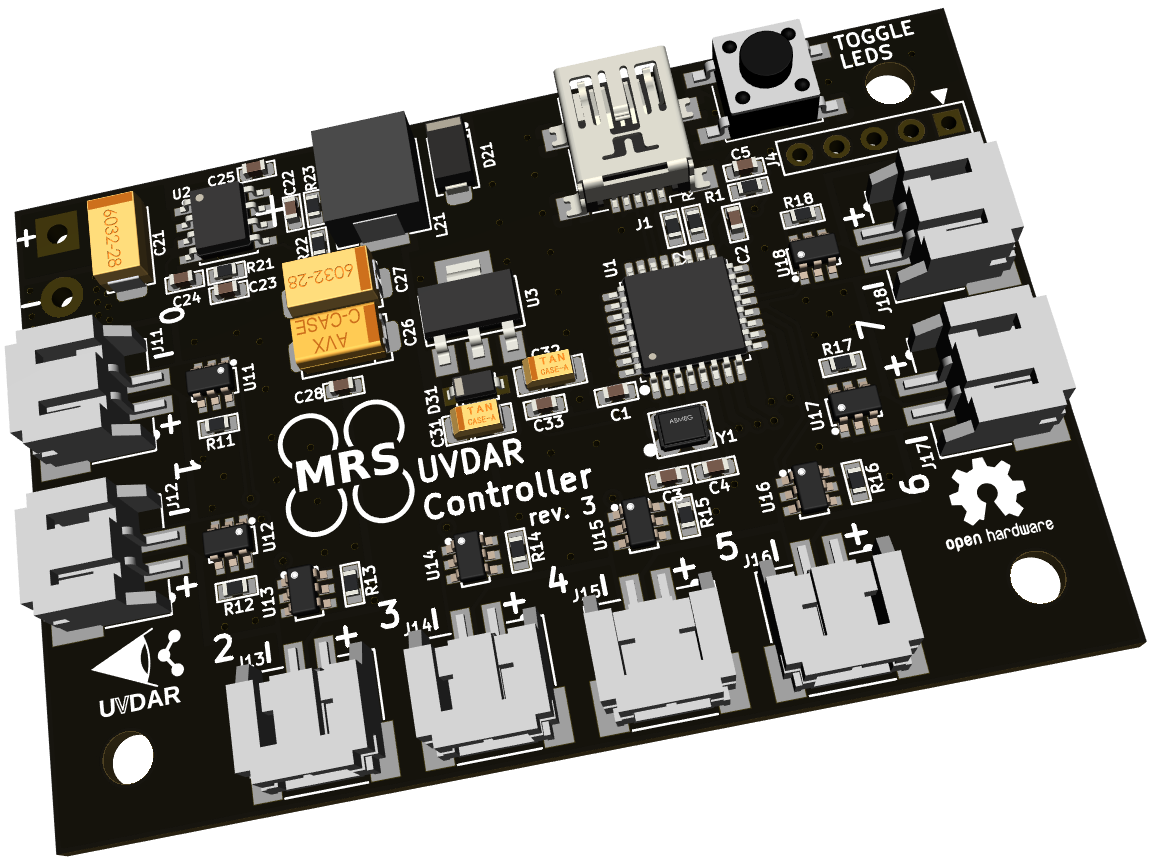
\includegraphics[width=0.9\textwidth]{figures/Thumbnail.png}
\caption{STANDALONE UVDAR CONTROLLER: Thumbnail}
\label{fig:thumbnail}
\end{figure}

\pagebreak
\subsection{Default Configuration}
The default configuration used by the MRS Group drives two UVLEDs ProLight Opto PM2B-1LLE per channel. These UVLEDs are soldered to a PCB which acts as a heatsink and mounting point to the end of the drone arm. The UVLEDs are at a right angle, which can be seen in figure \ref{fig:f450_with_uvdar}.\\\
\\
The voltage for UVLEDs is set to 8V, but this can be easily changed by adjusting the value of $R_{22}$ resistor according to the following formula:\\
$R_{22} = 22.1 \cdot \left(V_{OUT} - 1 \right) \left[ k\Omega \right]$
\\
The UVLEDs are driven using constant-current controllers that are set to approximately to 85mA. This value can be modified by changing the value of resistors $R_{11} - R_{18}$ according to the BCR421UW6 driver datasheet.\\
\\
Channels 1-4 are used to drive the UVLEDs on the arms and channels 5-8 are used to drive the beacon UVLEDs on the top of the drone.

\begin{figure}[h]
\centering
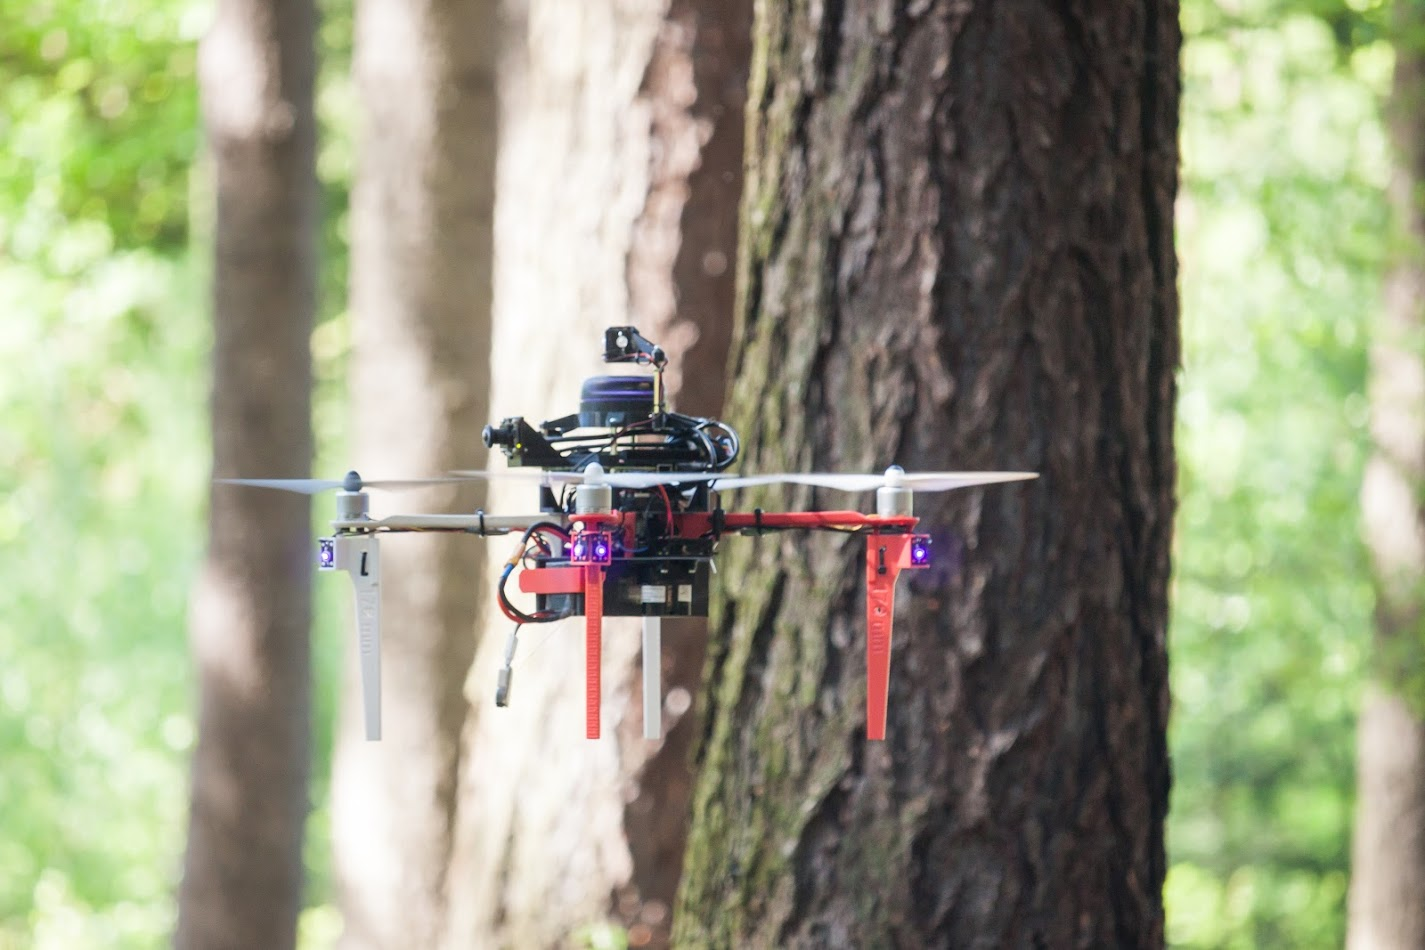
\includegraphics[width=0.9\textwidth]{figures/f450_with_UVDAR.jpg}
\caption{STANDALONE UVDAR CONTROLLER: Photo of an F450 drone with UVDAR}
\label{fig:f450_with_uvdar}
\end{figure}


\pagebreak
\section{Dimensions}
The Board is 67mm long and 45mm wide with three M3 mounting holes.\\
\\
The mechanical drawing can be seen in Figure \ref{fig:dimensions} below.

\begin{figure}[h]
\centering
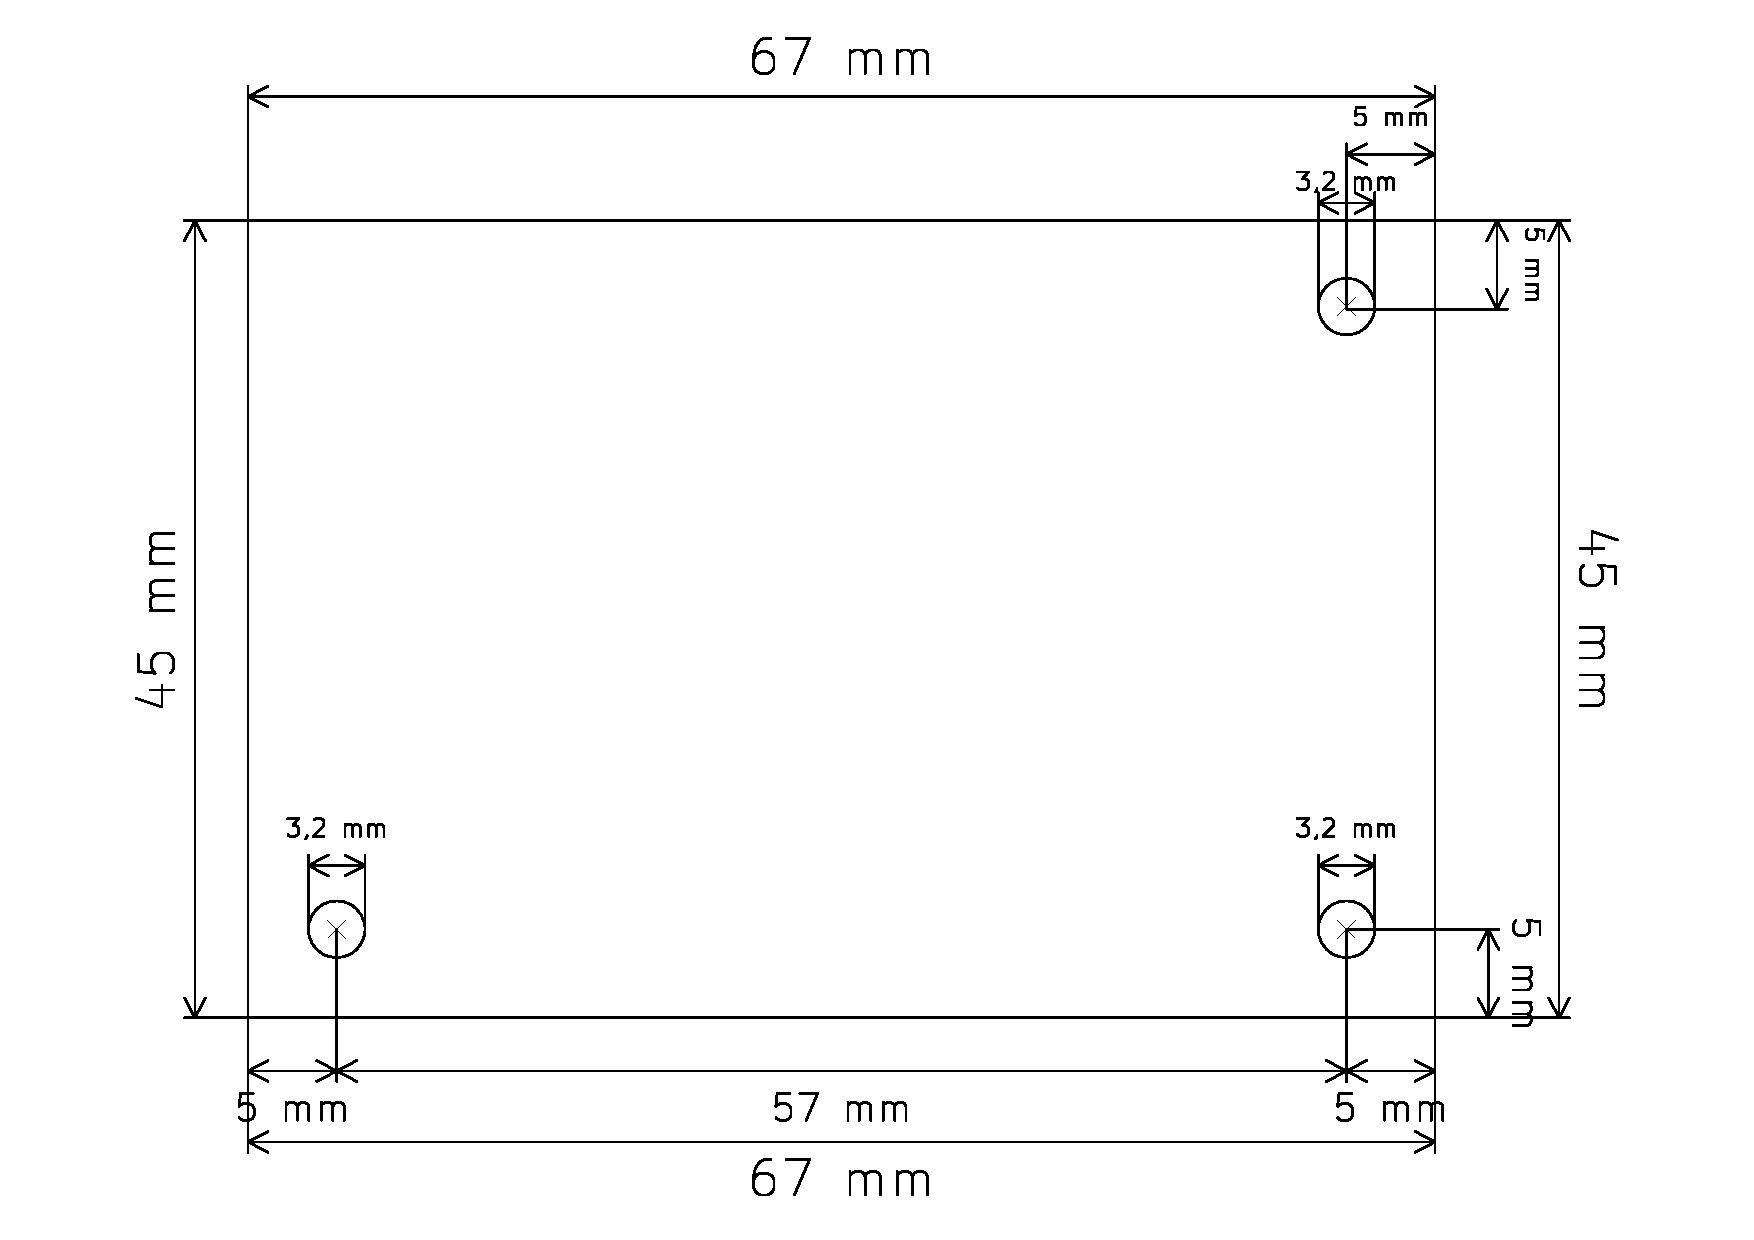
\includegraphics[width=\textwidth]{figures/Dimensions.pdf}
\caption{STANDALONE UVDAR CONTROLLER: Dimensions}
\label{fig:dimensions}
\end{figure}

\pagebreak
\section{Connectors}
The Board has 8 connectors numbered from 1 to 8 to connect UVLEDs. The pinout of these connectors is described in \verb|UVLED|.\\
The board has a connector for connecting to a Distribution Board with a standard pinout as seen in \verb|MRS MODULE|.\\
The last connector is the Serial Wire Debug (\verb|SWD|) connector for programming the on-board STM32F042K6T.
The connector placement can be seen in figures \ref{fig:connectors_top} and \ref{fig:connectors_bot}.
\subsection{Connector Placement Drawing}
\begin{figure}[h]
\centering
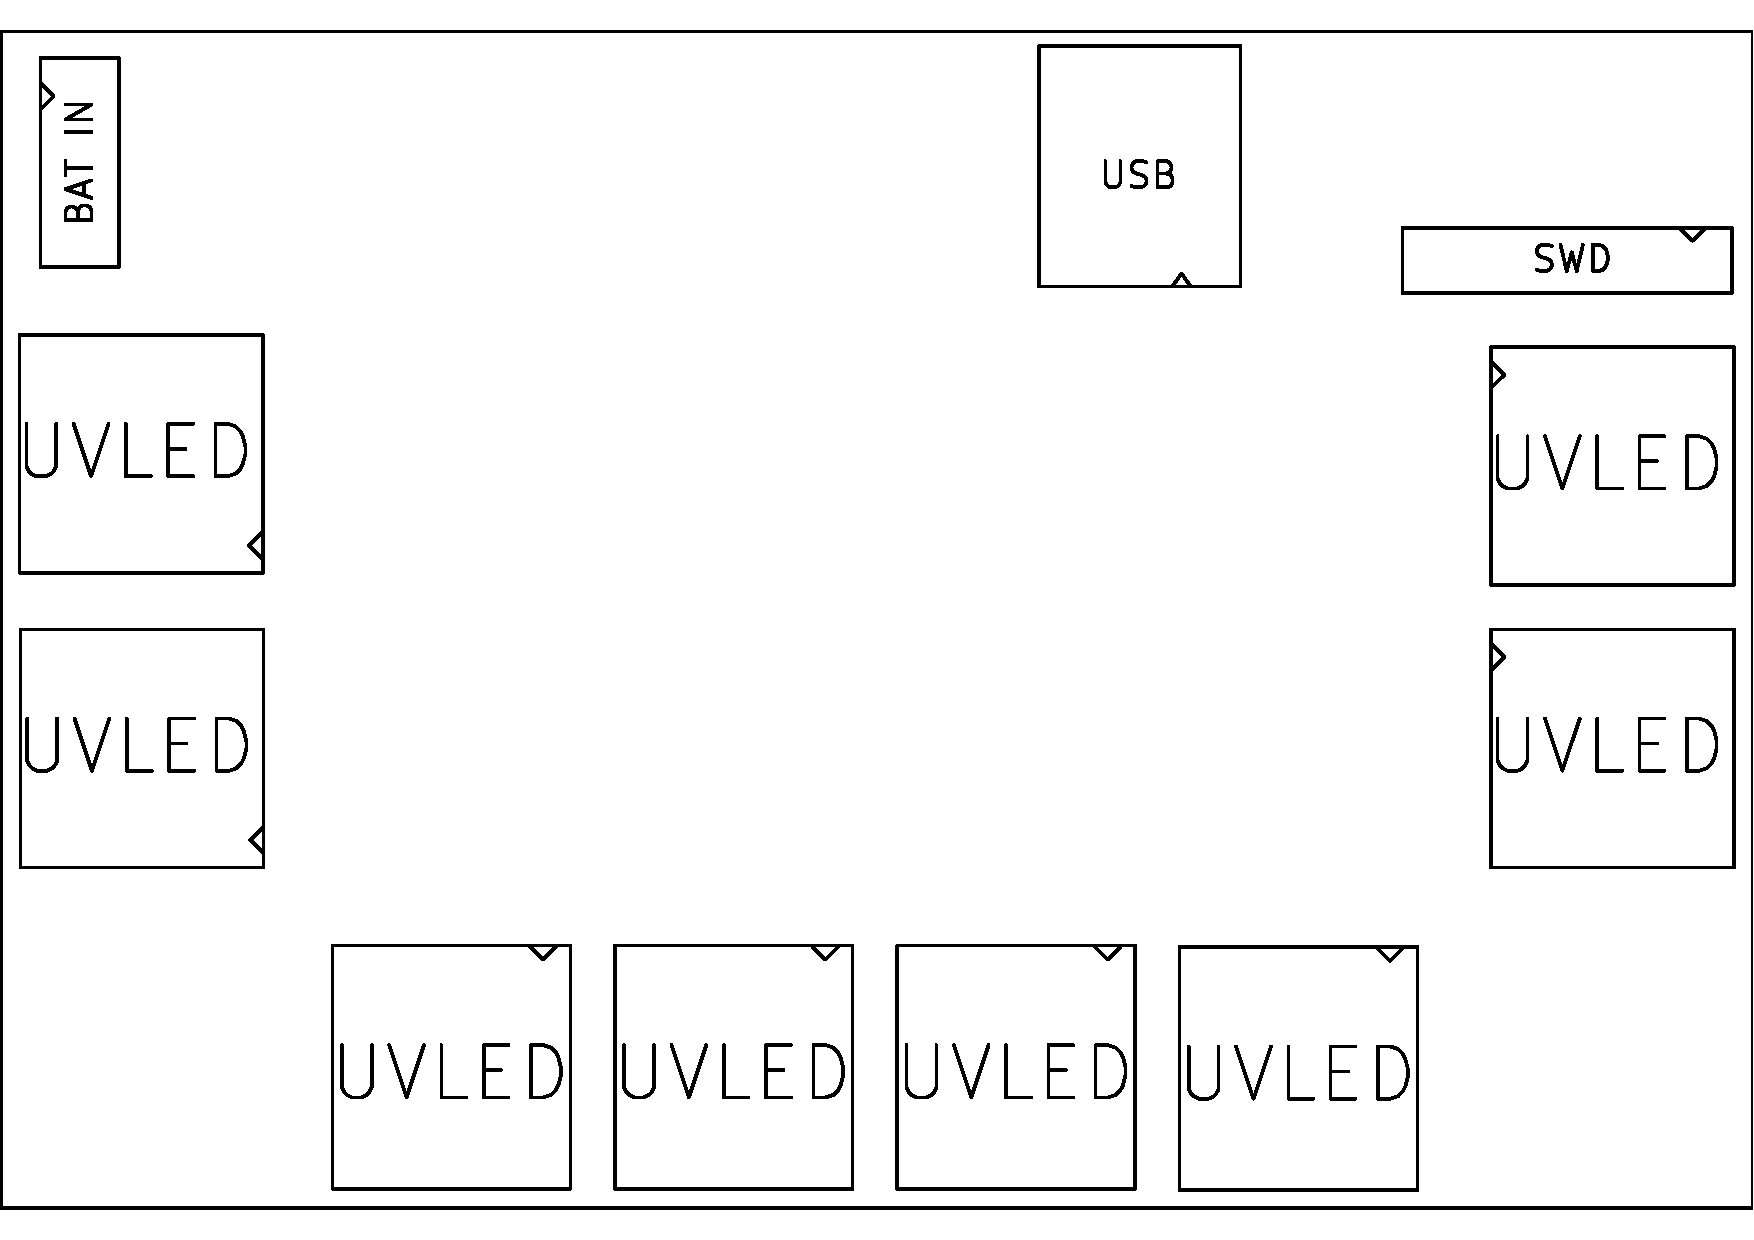
\includegraphics[clip=true,width=0.6\textwidth]{figures/Connectors_top.pdf}
\caption{STANDALONE UVDAR CONTROLLER: Connectors Placement, Top Layer}
\label{fig:connectors_top}
\end{figure}

\pagebreak
\subsection{Connector Pinouts}
\begin{center}
\begin{minipage}[t][3cm][t]{0.24\textwidth}
\centering
\begin{tabular}{|l|l|}
\hline
\multicolumn{2}{|p{2cm}|}{\centering\textbf{UVLED}} \\ \hline
1               & LED ANODE                \\ \hline
2               & LED KATHODE                \\ \hline
\end{tabular}
\end{minipage}
\begin{minipage}[t][3cm][t]{0.24\textwidth}
\centering
\begin{tabular}{|l|l|}
\hline
\multicolumn{2}{|p{2cm}|}{\centering\textbf{BAT IN}} \\ \hline
1               & BAT+                \\ \hline
2               & BAT-                 \\ \hline
\end{tabular}
\end{minipage}


\begin{minipage}[t][3.5cm][t]{0.24\textwidth}
\centering
\begin{tabular}{|l|l|}
\hline
\multicolumn{2}{|p{3cm}|}{\centering\textbf{USB}} \\ \hline
1               & VUSB         \\ \hline
2               & D-        \\ \hline
3               & D+        \\ \hline
4               & NC         \\ \hline
5               & GND     \\ \hline
\end{tabular}
\end{minipage}
\begin{minipage}[t][3cm][t]{0.24\textwidth}
\centering
\begin{tabular}{|l|l|}
\hline
\multicolumn{2}{|p{2cm}|}{\centering\textbf{SWD}} \\ \hline
1               & 3V3               \\ \hline
2               & SWCLK             \\ \hline
3               & GND               \\ \hline
4               & SWDIO             \\ \hline
5               & NRST              \\ \hline
\end{tabular}
\hfill
\end{minipage}

\begin{minipage}[t][3.5cm][t]{0.24\textwidth}
\centering
\begin{tabular}{|l|l|}
\hline
\multicolumn{2}{|p{3cm}|}{\centering\textbf{MRS MODULE}} \\ \hline
1               & GND         \\ \hline
2               & VBAT        \\ \hline
3               & VBAT        \\ \hline
4               & GND         \\ \hline
5               & UART\verb|_|TX     \\ \hline
6               & UART\verb|_|RX     \\ \hline
7               & GND         \\ \hline
8               & 5V          \\ \hline
9               & 5V          \\ \hline
10              & GND         \\ \hline
\end{tabular}
\end{minipage}
\end{center}

\pagebreak
\section{MCU Firmware}

The firmware receives data using USB; the data are in the \verb|baca_protocol| format used by the \verb|mrs_serial| node.\\
The button on the PCB serves to "mute" the UVLEDs. This button toggles global enable flag in order to stop the blinking, but does not change any other settings and does not stop the counter. This flag can be set using the UART as well.\\
\\
All setting are stored in the internal FLASH memory and are retrieved on startup.\\
\\
The byte structure of the \verb|baca_protocol| can be seen in table \ref{tab:baca_protocol_table}.
The message starts with letter 'b' (0x62 in hex) and is followed by the length of the payload (1-255).
The payload then follows. The first byte of the payload is the \verb|Message ID| and the rest of the payload contains the data (if any). The last byte is the checksum which is a simple sum of all previous bytes.\\
\\
Several message types have been implemented to control the board.

\begin{table}[h]
\begin{tabular}{|c|c|c|c|c|c|}
\hline
\textbf{Byte}   & 0          & 1                     & 2 ... (n-1) & n        \\ \hline
\textbf{Value} & 'b' (0x62) & Length of the payload & Payload (Message ID and Data)       & Checksum \\ \hline
\end{tabular}
\caption{STANDALONE UVDAR CONTROLLER: Baca Protocol Message}
\label{tab:baca_protocol_table}
\end{table}

\subsection{Message Types}
The available messages are described below:\\
\begin{itemize}
\item \textbf{Global Enable LEDs} - This is a software version of the HW switch on the PCB - This overrides, but saves all configuration and turns off all UVLEDs, or resumes the original settings.\\
\begin{flushleft}
\begin{tabular}{|l|}
\hline
Command Byte: 0x90													\\ \hline
Payload Size: 0														\\ \hline
\end{tabular}
\end{flushleft}

\item \textbf{Bulk Enable LEDs} - Enables or Disables the UVLED with the same index as the payload Byte. This will reset counters of all LEDs.\\
\begin{flushleft}
\begin{tabular}{|l|}
\hline
Command Byte: 0x91													\\ \hline
Payload size: 8 B													\\ \hline
Payload Bytes: 0x00 (UVLED Disabled), 0x01 (UVLED Enabled)			\\ \hline
Payload Byte 0: UVLED1 enabled =  0x00 (Disabled), 0x01 (Enabled)	\\ \hline
Payload Byte 1: UVLED2 enabled =  0x00 (Disabled), 0x01 (Enabled)	\\ \hline
Payload Byte 2: UVLED3 enabled =  0x00 (Disabled), 0x01 (Enabled)	\\ \hline
Payload Byte 3: UVLED4 enabled =  0x00 (Disabled), 0x01 (Enabled)	\\ \hline
Payload Byte 4: UVLED5 enabled =  0x00 (Disabled), 0x01 (Enabled)	\\ \hline
Payload Byte 5: UVLED6 enabled =  0x00 (Disabled), 0x01 (Enabled)	\\ \hline
Payload Byte 6: UVLED7 enabled =  0x00 (Disabled), 0x01 (Enabled)	\\ \hline
Payload Byte 7: UVLED8 enabled =  0x00 (Disabled), 0x01 (Enabled)	\\ \hline
\end{tabular}
\end{flushleft}

\item \textbf{Bulk Set Periods} - Sets blinking freqeuncy of the LED with the same index as the payload Byte. This will reset counters of all LEDs.\\
\begin{flushleft}
\begin{tabular}{|l|}
\hline
Command Byte: 0x92													\\ \hline
Payload size: 8 B													\\ \hline
Payload Byte 0: Desired frequency of the UVLED1						\\ \hline
Payload Byte 1: Desired frequency of the UVLED2						\\ \hline
Payload Byte 2: Desired frequency of the UVLED3						\\ \hline
Payload Byte 3: Desired frequency of the UVLED4						\\ \hline
Payload Byte 4: Desired frequency of the UVLED5						\\ \hline
Payload Byte 5: Desired frequency of the UVLED6						\\ \hline
Payload Byte 6: Desired frequency of the UVLED7						\\ \hline
Payload Byte 7: Desired frequency of the UVLED8						\\ \hline
\end{tabular}
\end{flushleft}

\item \textbf{Enable LED} - enables the UVLED with the specified index. This will reset the counter of the specified UVLED.\\
\begin{flushleft}
\begin{tabular}{|l|}
\hline
Command Byte: 0x93													\\ \hline
Payload Size: 2														\\ \hline
Payload Byte 0: UVLED index (0-7)									\\ \hline
Payload Byte 1: 0x00 (Disabled), 0x01 (Enabled)						\\ \hline
\end{tabular}
\end{flushleft}

\item \textbf{Set Period} - Sets blinking frequency of the UVLED with the specified index. This will reset the counter of the specified UVLED.\\
\begin{flushleft}
\begin{tabular}{|l|}
\hline
Command Byte: 0x94													\\ \hline
Payload Size: 2														\\ \hline
Payload Byte 0: LED index (0-7)										\\ \hline
Payload Byte 1: Desired frequency of the UVLED						\\ \hline
\end{tabular}
\end{flushleft}

\item \textbf{Get Enabled} - Returns 8 bytes. These bytes indicate if the UVLEDs are enabled or disabled.\\
\begin{flushleft}
\begin{tabular}{|l|}
\hline
Command Byte: 0x95															\\ \hline
Payload Size: 0																\\ \hline
Return Payload Size: 8														\\ \hline
Return Payload Byte 0: UVLED1 enabled =  0x00 (Disabled), 0x01 (Enabled)	\\ \hline
Return Payload Byte 1: UVLED2 enabled =  0x00 (Disabled), 0x01 (Enabled)	\\ \hline
Return Payload Byte 2: UVLED3 enabled =  0x00 (Disabled), 0x01 (Enabled)	\\ \hline
Return Payload Byte 3: UVLED4 enabled =  0x00 (Disabled), 0x01 (Enabled)	\\ \hline
Return Payload Byte 4: UVLED5 enabled =  0x00 (Disabled), 0x01 (Enabled)	\\ \hline
Return Payload Byte 5: UVLED6 enabled =  0x00 (Disabled), 0x01 (Enabled)	\\ \hline
Return Payload Byte 6: UVLED7 enabled =  0x00 (Disabled), 0x01 (Enabled)	\\ \hline
Return Payload Byte 7: UVLED8 enabled =  0x00 (Disabled), 0x01 (Enabled)	\\ \hline
\end{tabular}
\end{flushleft}

\item \textbf{Get Periods} - Returns 8 bytes. These bytes represent the frequency of the UVLEDs.\\
\begin{flushleft}
\begin{tabular}{|l|}
\hline
Command Byte: 0x96														\\ \hline
Payload Size: 0															\\ \hline
Return Payload Size: 8													\\ \hline
Return Payload Byte 0: UVLED1 Frequency									\\ \hline
Return Payload Byte 1: UVLED2 Frequency									\\ \hline
Return Payload Byte 2: UVLED3 Frequency									\\ \hline
Return Payload Byte 3: UVLED4 Frequency									\\ \hline
Return Payload Byte 4: UVLED5 Frequency									\\ \hline
Return Payload Byte 5: UVLED6 Frequency									\\ \hline
Return Payload Byte 6: UVLED7 Frequency									\\ \hline
Return Payload Byte 7: UVLED8 Frequency									\\ \hline
\end{tabular}
\end{flushleft}
\end{itemize}
\pagebreak
\subsection{Implementation notes}
The Board is equipped with the STM32F042K6T6 microcontroller. Its firmware is programmed using STM32Cube Hardware Abstraction Layer Libraries.\\
The pinout of the MCU can be seen in the Figure \ref{fig:ph_mcu_pinout}.\\
\begin{figure}[h]
\centering
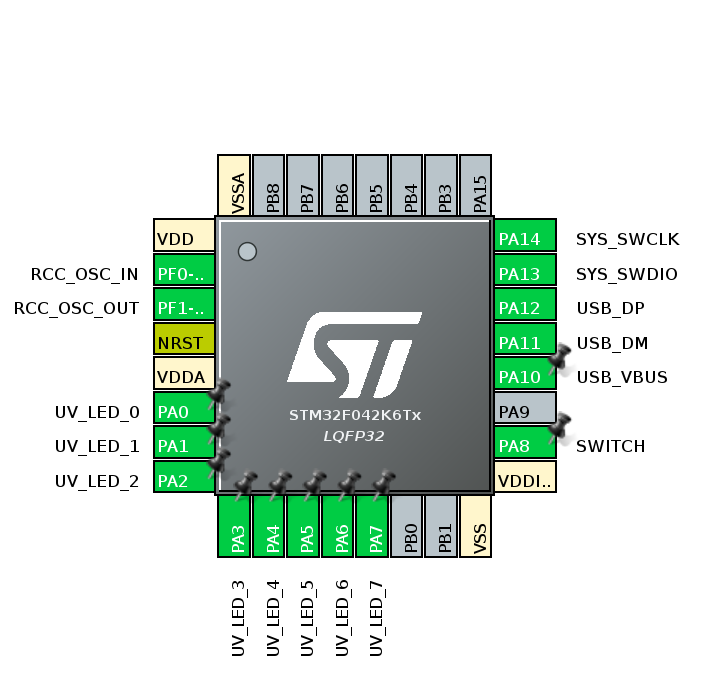
\includegraphics[width=0.9\linewidth]{figures/MCU_Pinout.png}
\caption{STANDALONE UVDAR CONTROLLER: MCU pinout}
\label{fig:mcu_pinout}
\end{figure}
The firmware is written with the need for versatility in mind and therefore is not optimal for specialised applications. The UVLED blinking is implemented using software PWM which allows us to change frequencies of individual channels, as is desired for research purposes. I suggest using hardware PWMs if the UVLEDs will have the same frequency. This is achievable only for UVLEDs 1 to 4 since these are connected to TIM2 channels 1 to 4. The other UVLED channels were moved to arbitrary pins for easier routing in the beginning and were left for legacy purposes. If hardware PWM for all channels is desired, then rearanging UVLEDs is necessary.

\pagebreak
\subsection{Software PWM for UVLEDs}
The UVLED blinking is implemented in \verb|uv_led_driver.c/h| files. To function properly, the pins must be named as \verb|UV_LED_x| where \verb|x| is a number between 0 and 8. This may of course be be changed by the programmer. These pins are used in the \verb|uv_led_init( void )| function to map them to an internally used array. This function also reads the frequency values and flags for enabling UVLEDs from the internal FLASH and resets the counters.\\
\\
The \verb|uv_led_set_frequency(uint8_t led_id, uint8_t frequency)| function sets the frequency of the selected UVLED. The input argument \verb|led_id| is index of the UVLED to be set starting from 0 and the \verb|frequency| is an integer value of desired frequency in range 1 to 60 Hz.\\
This function then calculates the number of ticks of the counter needed to toggle the LED (half of its total period). To calculate this value properly, the value of \verb|TIMER_FREQ| must be set to the frequency of the hardware timer used to increment the counter.\\
The calculated value is then saved to the internal FLASH.\\
\\
The \verb|uv_led_enable(uint8_t led_id, uint8_t enable)| function sets the enable flag of the selected UVLED. The input argument \verb|led_id| is index of the UVLED to be set starting from 0, with \verb|enable| as an integer of value 1 (true) or 0(false). Any other values are invalid.\\
The enable flag is then saved to the internal FLASH.\\
\\
The \verb|uv_led_toggle(uint8_t led_id)| function toggles the selected UVLED. The input argument \verb|led_id| is index of the UVLED to be set starting from 0.\\
This function is called if the counter value reaches the desired value. This is managed using the Timer Period Elapsed Callback Function \verb|HAL_TIM_PeriodElapsedCallback| where the counter is increased everytime the used timer's period elapses. The used timer in this appliation is \verb|TIM3| with a frequency of 10kHz.
\subsubsection{Global Enable Flag}
To be able to disable all UVLEDs on a button switch without affecting anything else, a simple flag was created. This flag toggles on with a button press (\verb|SWITCH|) or with receiving a global enable message using UART. This flag is used in the \verb|uv_led_toggle(uint8_t led_id)|.

\subsection{USB implementation}
TODO: Rewrite to USB
The USB communication using the STM Middleware. The message is processed in \verb|CDC_Receive_FS| function in \verb|usbd_cdc_if.c| file. If the message has the correct format (if the checksum is correct and has one of the valid message IDs), the apropriate function is called.\\
\\ VBUS Sensing has not yet been implemented.
\pagebreak

\newgeometry{left=1cm,right=1cm}
\section{Bill Of Materials and Assembly Drawings}
\begin{longtable}{|p{5cm}|p{5cm}|p{5cm}|p{1.7cm}|}
\hline
\textbf{References} & \textbf{Value} & \textbf{Footprint} & \textbf{Quantity}\\ \hline
C2, C5, C25, C33                       & 0.1uF                   & C0603                                      & 4        \\ \hline
C3, C4, C22                            & 10pF                    & C0603                                      & 3        \\ \hline
C1, C28                                & 1uF                     & C0603                                      & 2        \\ \hline
C23                                    & 1nF                     & C0603                                      & 1        \\ \hline
C24                                    & 10nF                    & C0603                                      & 1        \\ \hline
C31, C32                               & 10uF                    & CTAN1206                                   & 2        \\ \hline
C26                                    & 100uF/10V               & CTAN2312                                   & 1        \\ \hline
C21, C27                               & 22uF/25V                & CTAN2412                                   & 2        \\ \hline
R11, R12, R13, R14, R15, R16, R17, R18 & 3R3-0.5\%               & R0603                                      & 8        \\ \hline
R1, R2, R3, R22                        & 10k                     & R0603                                      & 4        \\ \hline
R21                                    & 27k4                    & R0603                                      & 1        \\ \hline
R23                                    & 1k1                     & R0603                                      & 1        \\ \hline
L21                                    & SRP6540-8R2M            & L\_SRP6540                                 & 1        \\ \hline
D21                                    & B340A                   & D\_SMA                                     & 1        \\ \hline
D31                                    & 1N4148W-E3-08           & SOD-123                                    & 1        \\ \hline
U1                                     & STM32F042K6T6           & LQFP-32\_7x7mm\_P0.8mm                     & 1        \\ \hline
U2                                     & TPS54331DR              & SOIC-8                                     & 1        \\ \hline
U3                                     & MCP1703-3302E           & SOT-223-3(TAB-pin-2)                       & 1        \\ \hline
U11, U12, U13, U14, U15, U16, U17, U18 & BCR421UW6               & SOT-26-6                                   & 8        \\ \hline
Y1                                     & ABM8G                   & ABM8G                                      & 1        \\ \hline
SW1                                    & Push-Switch\_SMT\_6x6mm & Tactile\_Switch\_6x6\_SMT                  & 1        \\ \hline
J4                                     & SWO                     & Header\_1x05\_P2.54mm                      & 1        \\ \hline
J11, J12, J13, J14, J15, J16, J17, J18 & JST-PH\_2               & JST\_PH\_2                                 & 8        \\ \hline
J1                                     & USB\_B\_Mini            & USB\_Mini-B\_Lumberg\_2486\_01\_Horizontal & 1        \\ \hline

\caption{STANDALONE UVDAR CONTROLLER: Bill Of Materials}
\label{tab:bom}
\end{longtable}
\vfill
\restoregeometry

\pagebreak
% change scale and angle accordingly
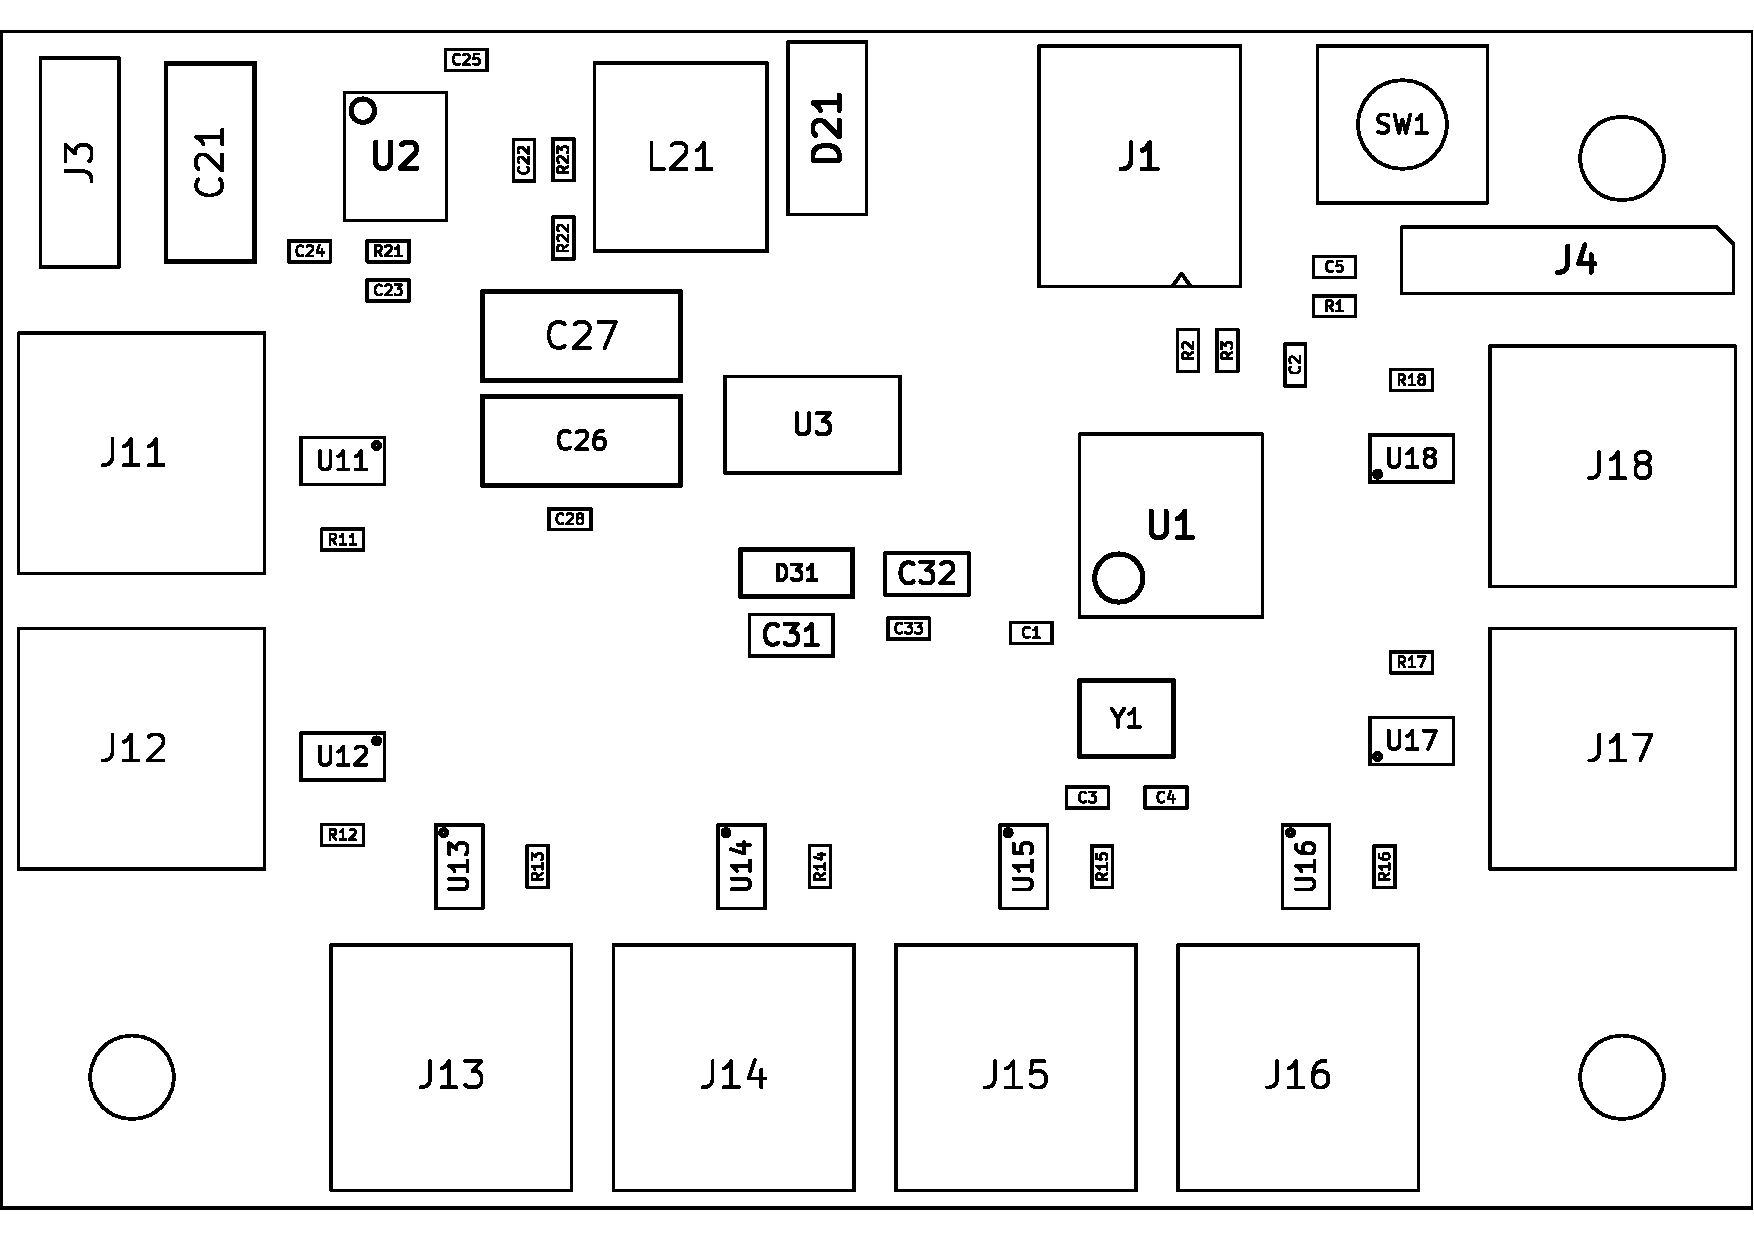
\includepdf[pages=-, scale=0.8, angle=270, pagecommand={}]{figures/Assembly_top.pdf}

\pagebreak
\section{Schematic}
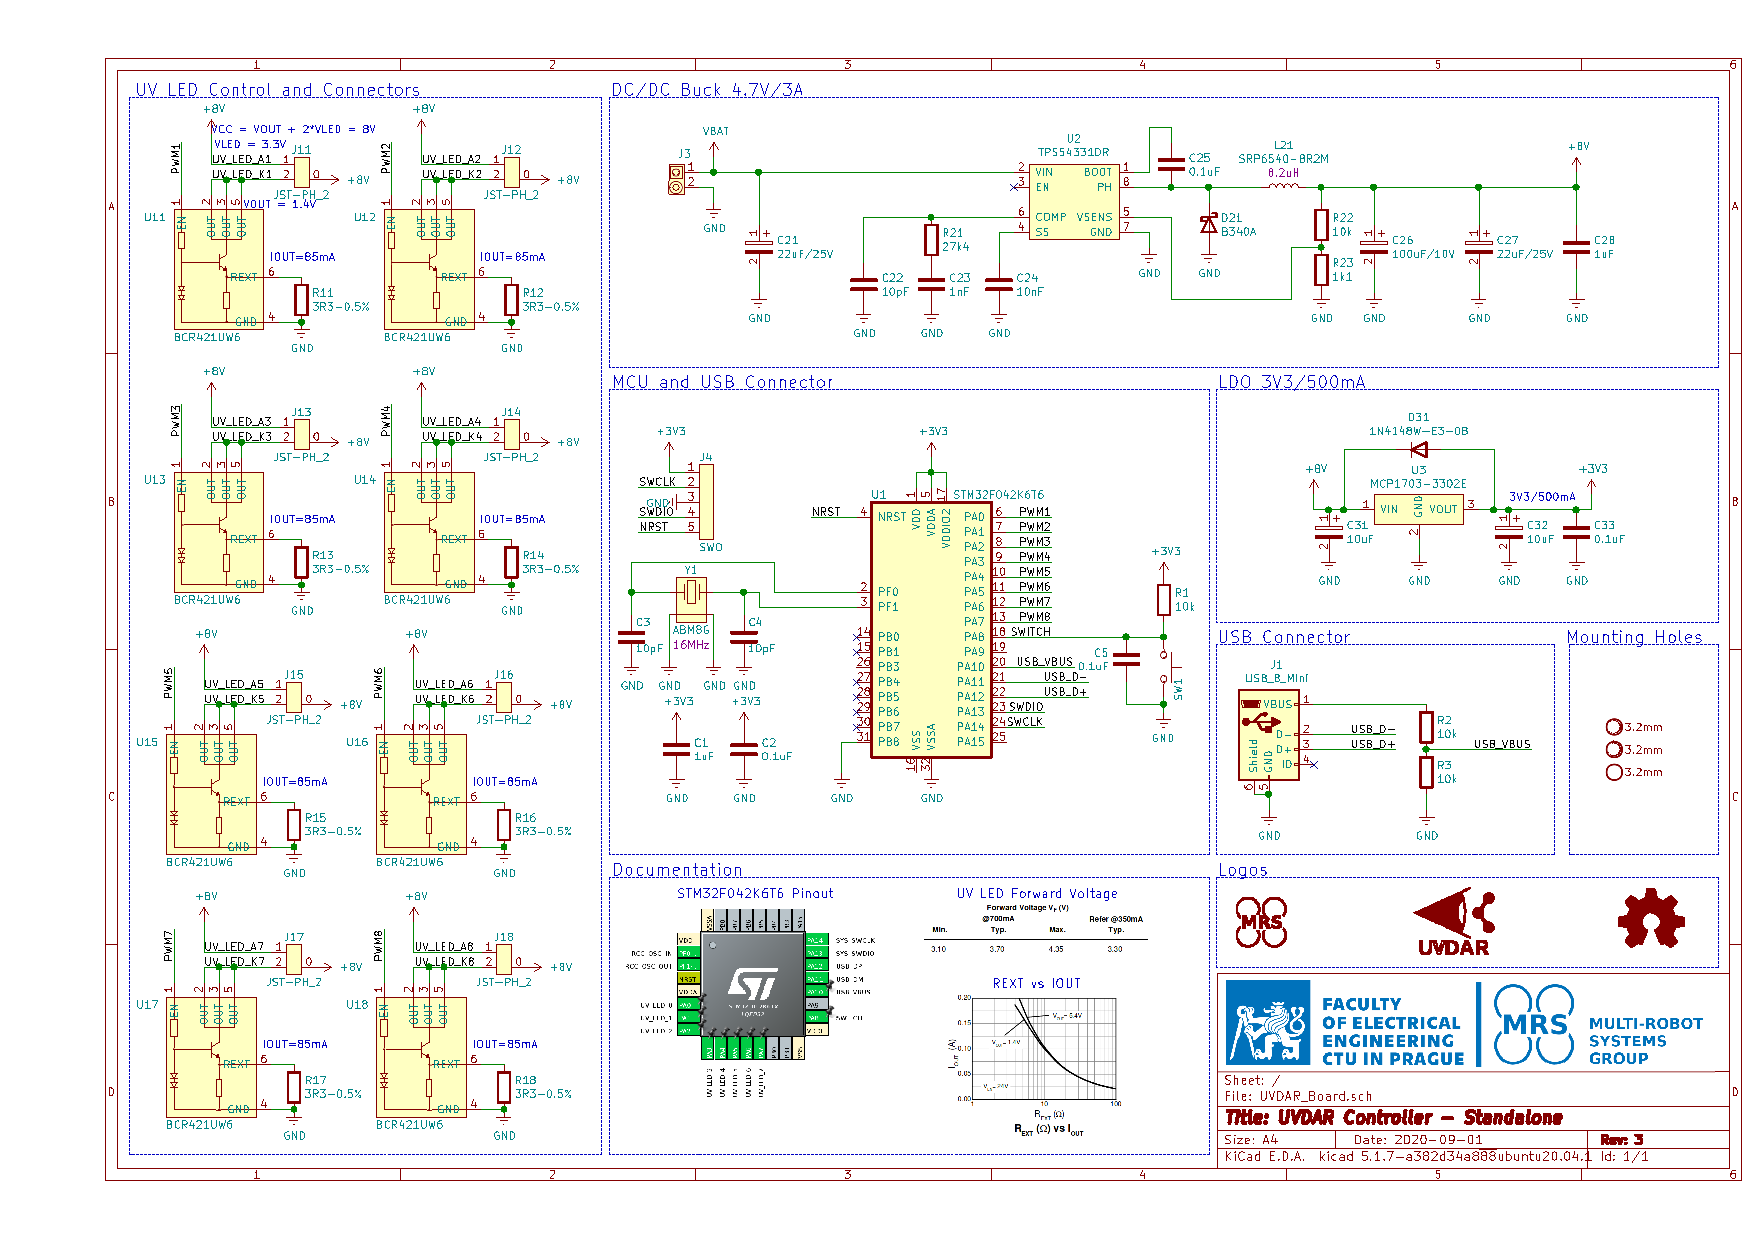
\includegraphics[scale=0.8, angle=270]{figures/Schematic.pdf}

\end{document}